%%%%%%%%%%%%%%%%%%%%%%%%%%%%%%%%%%%%%%%%%%%%%%%%%%%%%%%%%%%%%%%%%%%%%%%%%%%%%%%%
%2345678901234567890123456789012345678901234567890123456789012345678901234567890
%        1         2         3         4         5         6         7         8

\documentclass[letterpaper, 10 pt, conference]{ieeeconf}  % Comment this line out if you need a4paper
\usepackage{graphicx}
\usepackage{url}
\usepackage{multirow}
\usepackage{array}
\usepackage{courier}
\usepackage{url}
\usepackage{float}
%\documentclass[a4paper, 10pt, conference]{ieeeconf}      % Use this line for a4 paper

\IEEEoverridecommandlockouts                              % This command is only needed if
                                                          % you want to use the \thanks command

\overrideIEEEmargins                                      % Needed to meet printer requirements.



% See the \addtolength command later in the file to balance the column lengths
% on the last page of the document

% The following packages can be found on http:\\www.ctan.org
%\usepackage{graphics} % for pdf, bitmapped graphics files
%\usepackage{epsfig} % for postscript graphics files
%\usepackage{mathptmx} % assumes new font selection scheme installed
%\usepackage{times} % assumes new font selection scheme installed
%\usepackage{amsmath} % assumes amsmath package installed
%\usepackage{amssymb}  % assumes amsmath package installed

\title{\LARGE \bf
Generator for Academic Reports: Abstracts
}




\author{
	\begin{tabular}{*{2}{>{\centering}p{.5\textwidth}}}
		\large Daniel Christiani & \large Cody Smith \tabularnewline
		Computer Engineering & Computer Engineering \tabularnewline
		Rochester Institute of Technology & Rochester Institute of Technology \tabularnewline
		\url{dmc3413@rit.edu} & \url{cds7494@rit.edu}
	\end{tabular}
}


\begin{document}
\maketitle

\begin{abstract}
	Academic reports are extremely important and often serious documents. They report findings in an organized and referenceable way to inform, record, and shape our understanding of our world. For each domain of study, there are common structures in syntax and overall semantic flow of the article, specifically in the abstract. For this reason we will attempt to do a meta-analysis of academic papers and their abstracts in an effort to uncover the underlying semantic structure, syntactic preferences, and vocabulary of a given sub-domain and author of an academic community by designing an algorithm to generate new abstracts for reports given a training set.
\end{abstract}


\section{Introduction}

In this paper we describe an approach to generate academic report abstracts, given a corpus of abstracts to learn from.  The training abstracts are used to generate convincing academic abstracts for a given domain via an algorithm implemented in python. The algorithm uses a variety of natural language techniques including context-free grammar, n-gram analysis, and grammar equivalency to fill in a predetermined learned structure for an abstract in that domain. Related works include the SCIgen Automatic Computer Science Paper Generator\cite{jeremystribling2015}, which has successfully generated papers which were accepted at several conferences at the expense of organizers.

\section{Corpora}

To create a successful system, first corpora of different domain's abstracts needed to be created. For our purposes, it was important that the reports were sorted by domain, and that the topics of the papers were similar. While many different options were considered, to manage the data in a straight-forward manager, the abstracts were copied out of reports that were manually copied into plain text files. The directory structure for our corpus is shown in Figure \ref{fig:Directorystructure}.

\begin{figure}[!ht]
	\centering
	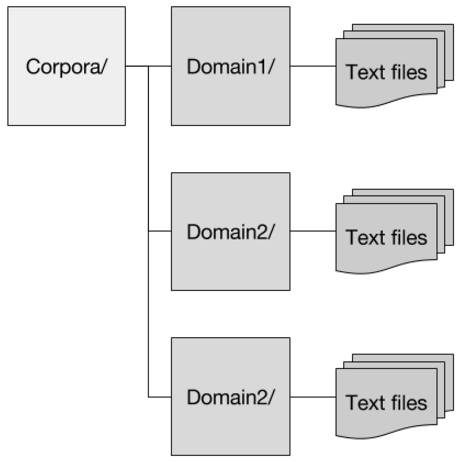
\includegraphics[width=.4\textwidth]{filestruct}
	\caption{Directory structure for the corpora.}
	\label{fig:Directorystructure}
\end{figure}


When accessing data from a corpus is required, the operation is as simple as looping over that directory and extracting the text from the text file. The code for doing that is shown in Figure \ref{fig:Codeparse}.  Any additional corpus added to a domain directory will automatically be processed as additional data. The next important step for this project is to preprocess the raw text from the abstracts. As described in the previous section, text is divided into sub directories where files contain individual abstracts.

\subsection{Preprocessing}

The first step in the preprocessing loads the text from a single corpora directory. For instance, choosing the directory ‘/computerscience’ will only load abstracts from the ‘Computer Science’ topic from which to preprocess text and eventually train our generator. Code is stripped of newline characters such that text will only be contiguous sentences.

When accessing data from a corpus is required, the operation is as simple as looping over that directory and extracting the text from the text file. The code for doing that is shown in Figure \ref{fig:Codeparse}. Any additional corpus added to a domain directory will automatically be processed as additional data.

\begin{figure}[!ht]
	\begin{verbatim}
	data = ""
	full_path = os.getcwd() + path
	for i in os.listdir(full_path):
	if i.endswith(".txt"):
	with open(full_path + '/' + i, 'r')
	as f:
	data += f.read().replace('\n', ' ')
	\end{verbatim}

	\caption{Code to parse corpus.}
	\label{fig:Codeparse}
\end{figure}

We created three total corpora, each for a different domain of different sizes and from different sources. Are hope was that by having different domains, sizes, and sources we would be able to evaluate our solution easier and that their differences would expose flaws or sucesses in the system.

\subsection{Computer Science Corpus}

The computer science corpus is a collection of 24 computer science paper abstracts. These were taken from the 2015 publications from Carnagie Mellon University (CMU), ranging from identifier CMU-CS-15-100 and on. Besides their shared domain, the authors and topics vary from papers about searching algorthms, statistics, vertual machines and more.

\subsection{Linguistics Corpus}

The linguistics corpus is a collection of 17 abstracts from mendeley.com, tagged with the topic linguistics. The filenames in the corpora folder are the ISSN. Besides the shared linguistics tag, each of the abstracts do not share authors or topics. The topics range from lexical semantics, speech and pronunciation, linguistic universals, visualizing linguistic data, and more.

\subsection{Nanocomputing Corpus}

The nanocomputing corpus is a collection on 13 abstracts from found Google scholar under Dr. Kudithapudi's page for published work\footnote{Works can be found at: \url{https://scholar.google.com/citations?user=RKGYlZEAAAAJ&hl=en&oi=ao}}. 

\section{Solution Overview}

The algorithm we developed is broken into three major parts. These parts include preprocessing, sentence generation, and scoring. An overview of each of these three steps is shown as Figure \ref{fig:SolutionOverview}.

\begin{figure*}[!ht]
	\centering
	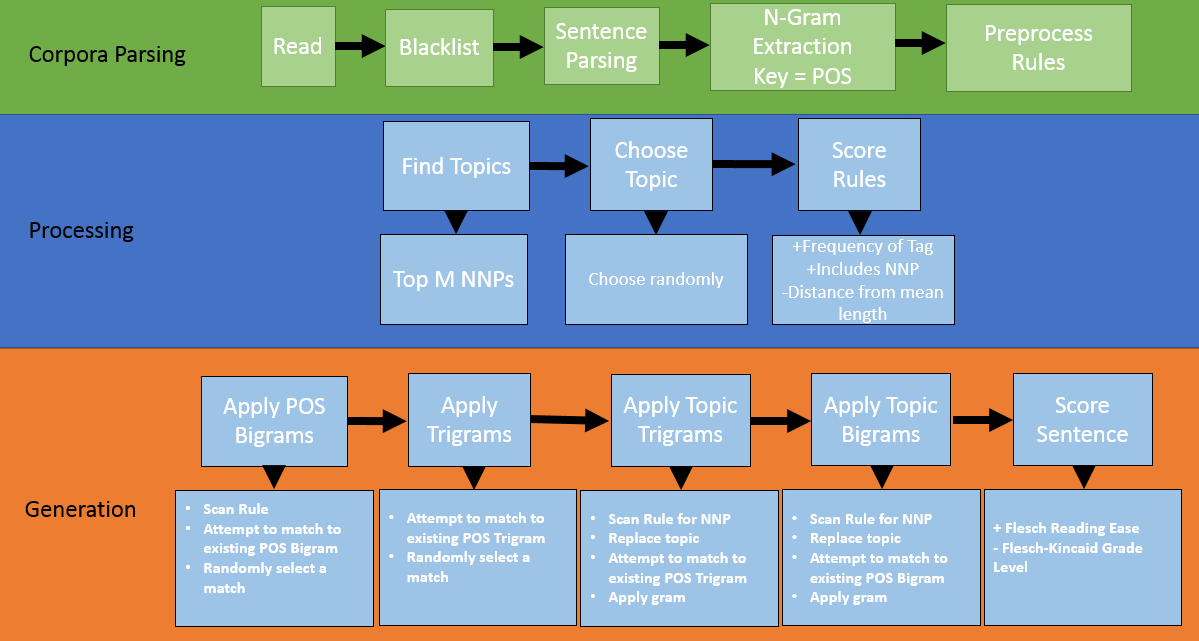
\includegraphics[width=1\textwidth]{overall_flow}
	\caption{Overall program flow. There are three primary stages: Corpra Parsing, processing, and generation. The parsing step is responsible for reading in the raw data, removing strange characters, parsing sentences, and creating the necessary data structures. The processing phase finds then chooses a topic for the abstract based on common proper nouns in the corpus, then scores a set of rules based on a number of criteria. Lastly, the generation takes those rules and creates sentences. Those sentences are then scored based on separate sentence criteria.}
	\label{fig:SolutionOverview}
\end{figure*}

\subsection{Preprocessing}

The first step in the preprocessing loads the text from a single corpus directory. For instance, choosing the directory ‘/computer\textunderscore science’ will only load abstracts from the ‘Computer Science’ topic from which to preprocess text and eventually train our generator. Each line is read and the newline characters are stripped such that text will only be contiguous sentences.

Once the read is complete, the raw text is stripped of all text in a blacklist. This blacklist contains characters such as quotes, parenthesis, and commas. Manual inspection of the text proved the blacklist to be critical to guarantee no unwanted special characters were included in the final data. It was decided to use a blacklist instead of a white-list because minus a couple of problematic characters, most punctuation seems to be valuable or at least has no negative consequence to the final result.

After the data is read in and the blacklist is stripped out, sentences are parsed. The parser moves over the text tokenizing every word and placing them into a list associated with a unique sentence. Decimal valued numbers are are found first with a regular expression, and are treated as individual tokens, otherwise, a string containing a period ‘.’ is considered the last word in the current sentence. The period is finally stripped from the sentence as clean tokenized words will be associated with our vocabulary. Future revisions may capture a variety of honorifics (e.g. ‘Dr.’) along associated with names of people as single tokens, however this is currently not supported.

The preprocessing of the raw data is now complete, however we must store this data in a way that we can utilize a form of context free grammar (CFG). The preprocessing stage stores parts-of-speech tags of the cleaned sentences, parts-of-speech tags of the vocabulary in a dictionary who's keys are the word's part-of-speech (POS) tags, as well as N-Grams and their respective parts of speech. For the abstract generator, 2-Grams, 3-Grams, and 4-Grams are collected.

\subsection{Rules}

For each sentence, a rule is created. These rules are a sequence of POS tags which generalize the structure of the sentence. The sentences are POS tagged using NLTK's POS tagger, and utilize Penn's Treebank tags. These rules will sometimes contain either undesirable structures, incorrect tags, or other issues so to sort the good rules from the bad, the rules are scored. Starting with a score of zero, positive and negative features are calculated against the rule. Positive features include the number of occurrences of the most common corpus tags. Negative features include the difference in the length of the rule from the mean length of all sentences in the corpus. These rules are then sorted by their score, so that the best n rules can be used to generate n sentences.

\subsection{Topic Selection}

For each generated abstract, a topic must be chosen. This topic represents the main subject for the paper, and is chosen from the corpus. To chose a topic, first the corpus's NNP tags are sorted by frequency. The NNP tag is the Treebank tag for singular proper nouns, which often work well as topics. From the top 10 most frequent NNPs, a topic is then chosen randomly picked. This topic then becomes preferentially added to generated sentences during their creation.

\subsection{Sentence Generation}

To generate a sentence, the first step is to select a rule. For our algorithm, we start with the highest scoring rule for the first sentence and continue to move down the list as more sentences are generated. After a rule is selected, it then goes through a couple of stages.

The first is applying bigrams. From left to right, bigrams are applied for each part of speech in the rule. Often times, there are more than one options for which words to use for a part of speech. For efficiency reasons, one and only one is selected randomly from the possible options, and then we continue until the rule is complete. The second step is similar the first, expect this time with trigrams. Selectively, trigrams are applied to the sentence from left to right, and when there are multiple options one is selected randomly. The processes is repeated again, expect this time only for rules involving NNP tags, for the purpose of inserting the topic of the abstract into the structures. First from left to right where possible the bigrams with NNPs in the sentence are replaced with the topic chosen earlier. Then again the process is repeated with trigrams to replace the NNPs in the sentence with the topic. At this point the generated sentence is ready to scored and potentially used.

\subsection{Sentence Scoring}

After the sentences are generated, selecting which sentences will be used in the abstract is done just like the rules with scoring. There are positive and negative features chosen to separate good sentences from bad, and each generated sentence is scored against these features. For sentences, positive features include the Flesch-Kinacaid reading ease. The Flesch-Kinacaid reading ease\cite{flesch1948new} is a measure of how easy a selection of text is to read, and is calculated with the formula shown as in  Equation \ref{eq:1}.

\begin{equation} \label{eq:1}
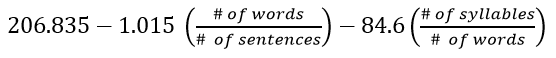
\includegraphics[width=.4\textwidth]{ease_eq}
\end{equation}

Negative features include duplicate words in a row which has a very steep penalty, and the Flesch-Kinacaid grade level \cite{si2001statistical} as in  Equation \ref{eq:2}. The Flesch-Kinacaid grade test is a way to calculate the US school system grade level for a passage. In this case lower is a lower grade level and therefore easier to understand.

\begin{equation} \label{eq:2}
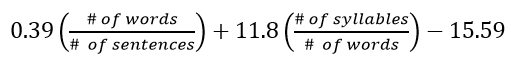
\includegraphics[width=.4\textwidth]{grade_eq}
\end{equation}

All of these positive and negative features are added together to form a total score for each generated sentence. This score is used to sort the sentences, and the top sentences are chosen to generate an abstract with.

\section{Results and Summary}

This algorithm as described was implemented in python, and is open source and viewable on GitHub\footnote{GitHub Link to Project Directory:  \url{https://github.com/codysmithd/ARAG}}. Due to time constraints, many details of the implementation are not ideal, however the algorithm was used successfully to generate many abstracts for evaluation. Once these abstracts were being generated for the given domains, we then took a sample and evaluated them to examine how successful we were.

\subsection{Evaluation Criteria}

There are many challenges with evaluating the generated abstracts, especially surrounding quantifying how successful they are. However, as some form of evaluation is required to make sense of our results, we designed two methods to evaluate abstracts. The first is the number of edits required to make the generated abstracts grammatically correct. The second is the the number of edits needed to make the report semantically correct. Both of these measure a single edit as a contiguous change made to the abstract.


\subsection{Example Abstract}

To illustrate how the abstracts are scored, the following is an actual example generated abstract, with one evaluator's syntax and semantic corrections. The chosen subject of the abstract is `graphs`.
\begin{figure}[!ht]
\small
\texttt{ We present the acid arms of graphs and b-a algorithms property of graphs design in a contextual. We learn these transition aspects of graphs and coordinate graphs key part of the part of the interplay. Graphs simulation data to integrate properties in key of being bound and graphs by building initiated as queries. Graphs are methods to perform creators in general by being programmed and instead of existing case of businesses. Of this latter we investigate design images to real approximate ideas in graphs and nonparanormal model improvements as graphs spatial-connectivity and productivity.}
	\caption{Raw output from abstract generator.}
	\label{fig:example_output_raw}
\end{figure}
\normalsize
\noindent
After an evaluator attempted to fix the grammar of the generated abstract, a total of 7 edits where made. The result was as follows:
\noindent
\begin{figure}[!ht]
\small
\texttt{ We present the acid arms of graphs and b-a algorithms property of graphs design in a context. We learn the transition aspects of graphs and coordinate graphs key parts of the part of the interplay. Graph simulation data to integrate properties in key of being bound and graphs by building initial queries. Graphs are methods to perform creators in general by being programmed and instead of existing case of businesses. Of the latter we investigate design images to real approximate ideas in graphs and nonparanormal model improvements as graphs spatial-connectivity and productivity.}
	\caption{Raw output from abstract generator.}
	\label{fig:example_output_grammar}
\end{figure}
\normalsize

It should be noticed that at this point the semantics of the abstract are very much still not ideal. Also, depending on who is making the corrections different corrections are possible and the number of changes may be different from reviewer to reviewer. Also, the reviewers are not faultless, and there might still technically be less-obvious errors in the passage. To fix the semantics one reviewer edited the abstract with 25 edits; the result can be seen in Figure \ref{fig:example_output_grammar_two}
{
\noindent
\begin{figure}[H]
\small
\texttt{ We present graphs and b-a algorithms. We learn the transition aspects of graphs and coordinate graphs key parts. Graph data integrates properties of being bound as queries. Graphs are methods to perform analysis in general by being programmed. We investigate design images to approximate ideas in graphs and nonparanormal model improvements as graphs spatial-connectivity and productivity.}
\caption{Raw output from abstract generator.}
\label{fig:example_output_grammar_two}
\end{figure}
\normalsize
}

Most of the edits to the abstract were deleting text with only a single word added, and otherwise the changes were minimal. The core content of the generated abstract was maintained and this is perhaps validation of the original concept for the generator.

\subsection{Analysis of Different Evaluators}

To quantify the differences and challenges with using human evaluators, the authors of this paper both evaluated a selection of passages. Two evaluators were selected to modify the raw abstracts until they were both readable, and made logical sense. The evaluators were asked to keep track of the two primary evaluation criteria while performing these corrections.

\begin{figure}[!ht]
	\centering
	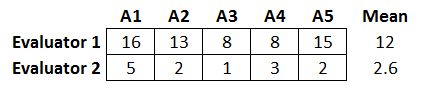
\includegraphics[width=.4\textwidth]{grammer_result}
	\caption{Results from human grammar correction for two examiners on five different abstracts.}
	\label{fig:grammarresult}
\end{figure}

The results from grammar are seen in Figure \ref{fig:grammarresult}. Five random abstracts were chosen to evaluate that were either generated from the Computer Science, Linguistics, or Nanocomputing corpora. Two evaluators then corrected the abstract. Using the same evaluators and the now grammar corrected abstracts, the text was then corrected for semantic sense. The amount of these corrections is tabulated in Figure \ref{fig:semanticresult}.

\begin{figure}[!ht]
	\centering
	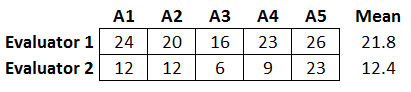
\includegraphics[width=.4\textwidth]{semantic_result}
	\caption{Results from human semantic correction for two examiners on five different abstracts.}
	\label{fig:semanticresult}
\end{figure}

The amount semantic corrections per abstract averaged much higher than the number of grammatical corrections per abstract for both evaluators. This was to be expected as semantically correct text requires a lot of corrections until the text makes logical sense. It also can be noted that for certain abstracts, proportionally less work was needed to correct it for both evaluators. From this we can draw two observations: certain abstracts are of higher quality then others and although it took proportionally less work, one evaluator required more corrections. This leads to an issue when evaluating the text as some people will be naturally more critical of the text then others, however we can still uncover trends in the overall quality of the text in terms of which abstracts required more or less corrections across multiple users. For example if we add the semantic and grammatical scores for each corpus by evaluator, we can rank the abstracts by level of quality. In that case, we rank the abstracts as A3 having the lowest score, followed by A4, A2, A1, then A5 having the highest score and therefore the lowest quality. This quality list is true for both evaluators and therefore seems to be an effective scoring method.



\subsection{Results Observations}

There were many observations made about the generated abstracts during their evaluations. The first is that the size of the corpus made a large difference in the results. The computer science corpus had the most abstracts and also seemed to perform the best. Also, topic selection is an important step. Reports with bad topic selection did not have good results, where good topics generally had better results.

\subsection{Future Improvement}

While there are many aspects of the algorithm and it's results that exceeded expectations, through the process of creating this system there were many things that showed promise as areas that could be improved. These improvements break down into several major categories.

\subsubsection{Corpora}

During the development of the algorithm, it became very clear that a larger corpus of abstracts lead to much better results. While there was a cost to processing time, having more vocabulary, more n-grams, and more structures lead to much better generated abstracts. In the future it would be nice to test the algorithm against significantly larger corpora. It also became clear that
when the corpus had a single style, author, or otherwise similar data the results where also better. With that observation it would be nice in the future to improve the corpora by sorting by topic or author to make generated abstracts have a more consistent feel.

\subsubsection{Performance}

The design of the algorithm lends itself to being able to be completed as a series of parallel tasks. However, our implementation was not able to take advantage of this due mostly to time constraints, so increasing the performance by utilizing parallel computing techniques would be a great next step. Also, many individual tasks in the algorithm were also implemented in non-performant ways for the sake of getting completed and tested first, so being able to go back and re-design some of the sub-steps would be a good next step.

\subsubsection{Scoring}

The idea behind scoring at different levels of the generation process was very crucial to the success of this algorithm, and the use of scoring in the future would be recommended. However, the use of scoring for this paper is limited to one or two simple positive and negative features. In the future, taking advantage of more advanced scoring techniques as well as how other layers of the process can be scored, sorted, and evaluated to reduce the amount of work necessary to get a good result would be recommended.

\subsubsection{Part of Speech Tagging}

The Penn Treebank POS tagger that was used in this paper was for the most part successful. However, Adding tags for the start and end of sentences was an idea that was considered but not implemented for this report. Adding this layer into the bigrams and trigrams could serve useful in the future to make the starts and ends to the sentences be less troublesome.

\subsubsection{Machine Learning}

The role of a more traditional context-free grammar (CFG) system was how this project was started, however due to it's poor performance it was abandoned in favor of single-sentence rules that are one level deep. Be re-evaluating the roll of CFG and creating larger and better structured trees, perhaps through machine learning might offer a way to improve the results of the system. Also, machine learning could be utilized to improve scoring, and many other aspects of the algorithm.

\section{Conclusion}

Through a combination of techniques individual sentences that are characteristic of a corpus can be generated. These sentences, if carefully selected, can be arranged intelligently to form more complete documents. By training a system on report abstracts, this system is able to use the content and structure of the abstracts to generate new abstracts with topics chosen from nouns in the corpus. With relatively minimal editing these generated abstracts can be made grammatically and semantically correct.

\addtolength{\textheight}{-12cm}   % This command serves to balance the column lengths
                                  % on the last page of the document manually. It shortens
                                  % the textheight of the last page by a suitable amount.
                                  % This command does not take effect until the next page
                                  % so it should come on the page before the last. Make
                                  % sure that you do not shorten the textheight too much.

%%%%%%%%%%%%%%%%%%%%%%%%%%%%%%%%%%%%%%%%%%%%%%%%%%%%%%%%%%%%%%%%%%%%%%%%%%%%%%%%



%%%%%%%%%%%%%%%%%%%%%%%%%%%%%%%%%%%%%%%%%%%%%%%%%%%%%%%%%%%%%%%%%%%%%%%%%%%%%%%%



%%%%%%%%%%%%%%%%%%%%%%%%%%%%%%%%%%%%%%%%%%%%%%%%%%%%%%%%%%%%%%%%%%%%%%%%%%%%%%%%




%%%%%%%%%%%%%%%%%%%%%%%%%%%%%%%%%%%%%%%%%%%%%%%%%%%%%%%%%%%%%%%%%%%%%%%%%%%%%%%%




%\begin{thebibliography}{99}

%\bibitem{c1} M. Romay, 'Hyperspectral Remote Sensing Scenes - GIC', Ehu.eus, 2015. [Online]. Available: http://www.ehu.eus/ccwintco/index.php?title=Hyperspectral_Remote_Sensing_Scenes. [Accessed: 26- Oct- 2015].



\bibliographystyle{plain}
\bibliography{citations}

%\end{singlespace}




%\end{thebibliography}




\end{document}
